\chapter{Herramientas}
\label{chap:herramientas}
En este capítulo se van a detallar las herramientas utilizadas en el desarrollo de este proyecto. Algunas se han elegido por facilidad de uso y otras por necesidad del entorno desarrollado.

% JAVASCRIPT %
\section{JavaScript}
\label{sec:js}
\textit{JavaScript} es un lenguaje interpretado de alto nivel que se encuentra bajo el estándar \textit{ECMAScript}\footnote{Especificación de lenguaje de programación el cual define tipos dinámicos y soporta características de programación orientada a objetos.} y está basado en otros lenguajes de programación como Java o C. 

En su principio fue concebido como lenguaje para el lado cliente implementado en un navegador web, permitiendo mejorar la interfaz de usuario y realizar páginas web dinámicas. 
Actualmente, JavaScript se ha ido integrando en el lado servidor y es por ello que es el lenguaje más utilizado para desarrollo web y todos los navegadores interpretan el código integrado en las páginas web.
\subsection{Características}
Las siguientes características tienen en común que todas se ajustan al estándar de ECMAScript: 
\begin{itemize}
    \item Es un lenguaje estructurado, tiene gran similitud con \textit{C} y comparte gran parte de su estructura (bucles, condicionales, sentencias...) a excepción del alcance de sus variables. En \textit{C} su ámbito es el bloque en el que fue definida y, en su origen, \textit{JavaScript} tenía un alcance global en las variables definidas. Es en ECMAScript 2015 cuando se añade la palabra clave \textit{let}, que incorpora compatibilidad con \textit{block scoping}(alcance de la variable en el bloque en la que es definida). 
    \item Tipado débil, por el cual el tipo de datos está asociado al valor, no a la variable. Esto significa que una variable puede ser \textit{number} o \textit{string} en distintos momentos de ejecución. 
    \item Formado en su totalidad por objetos, en los cuales los nombres de sus propiedades son claves de tipo cadena siendo \textit{objeto.a = 1} y \textit{objeto['a'] = 1} equivalentes. 
    \item Lenguaje interpretado, es por esto que no requiere un compilador ni crear un fichero binario del código; cada navegador tiene su intérprete que se encarga de ejecutarlo.
    \item Evaluación en tiempo de ejecución gracias a la función \textit{eval}, la cual evalúa un código en \textit{JavaScript} representado como una cadena de caracteres. 

    
\end{itemize}
% A-FRAME %
\section{A-Frame}
\label{sec:aframe}
A-Frame es un framework de código abierto destinado a crear experiencias de realidad virtual a partir de \textit{HTML} de forma que sea sencillo de leer y comprender. De esta manera es accesible para crear una gran comunidad. 


Además tiene compatibilidad con \textit{Vive}, \textit{Rift}, \textit{Windows Mixed Reality}, \textit{Daydream}, \textit{GearVR} y \textit{CardBoard} así como soporte para todos los controladores respectivos. También ofrece soporte para ordenadores de escritorio y para la mayoría de teléfonos inteligentes.

\subsection{HTML y primitivas}
\textit{A-Frame }se basa en \textit{HTML} y el \textit{DOM} usando un \textit{polyfill}\footnote{Fragmento de código en \textit{JavaScript} utilizado para proporcionar una funcionalidad moderna en navegadores antiguos.} para elementos personalizados. \textit{HTML} es un componente básico para Web y como tal, tiene una gran accesibilidad como lenguaje. Para crear una escena de realidad virtual con \textit{A-Frame} no se requiere ninguna instalación y simplemente con la creación del \textit{HTML} se puede abrir en el navegador. La mayoría de herramientas existentes(como \textit{React}, \textit{Vue.js}, \textit{d3.js} y \textit{jQuery}) funcionan en este framework. 

\textit{HTML} y \textit{DOM} son solo la capa más externa del framework, debajo se encuentra el componente \textit{three.js} en el que está basado \textit{A-Frame} gracias al cual un componente puede ser utilizado en distintas entidades. De esta manera hace posible seguir el principio de programación \textit{Don't Repeat Yourself} ya que, una vez registrada una primitiva, se puede hacer referencia al elemento todas las veces que sea necesario.  

A-Frame proporciona elementos como \textit{a-box} o \textit{a-sky} llamados primitivas. Podemos crear un escenario a través de estas primitivas como el mostrado en la figura \ref{fig:scene1} con el siguiente código: 

\begin{lstlisting}[language=javascript, caption=Código con primitivas que representa un escenario]
<!DOCTYPE html>
<html>
  <head>
    <meta charset="utf-8">
    <title>Escenario primitivas</title>
    <script src="https://aframe.io/releases/0.9.2/aframe.min.js"></script>
  </head>
  <body>
    <a-scene background="color: #FAFAFA">
      <a-box position="-1 0.5 -3" rotation="0 45 0" color="#4CC3D9" shadow></a-box>
      <a-sphere position="0 1.25 -5" radius="1.25" color="#ff0000" shadow></a-sphere>
      <a-cylinder position="1 0.75 -3" radius="0.5" height="1.5" color="#FFC65D" shadow></a-cylinder>
      <a-plane position="0 0 -4" rotation="-90 0 0" width="4" height="4" color=" #1cde83" shadow></a-plane>
      <a-sky color="#e7e1e0"></a-sky>
    </a-scene>
  </body>
</html>
\end{lstlisting}

\begin{figure}[H]
\centering
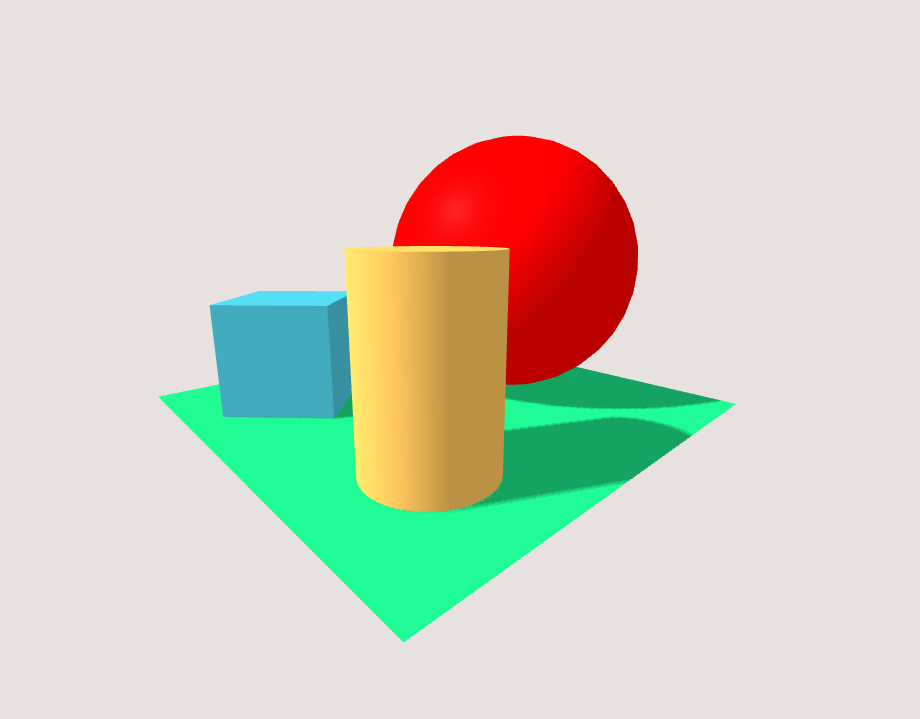
\includegraphics[width=0.8\textwidth]{img/scene1.png}
\caption{Escenario a-frame} \label{fig:scene1}
\end{figure}

A-Frame, además de disponer primitivas como las mostradas, hace posible la creación de primitivas para poder elaborar escenas lo más completas posible. También se pueden incluir entidades más complejas a partir de modelos 3D en formatos como \textit{gltf}, \textit{obj} o \textit{collada} de los cuales se hablará en siguientes apartados.

\subsection{Entidad, Componente y Sistema}

    Como ya se ha comentado, A-Frame es un framework \textit{three.js} con una arquitectura de entidad-componente-sistema (\textit{ECS}). Es un patrón común en 3D y desarrollo de juegos que siguen la composición sobre el principio de herencia y jerarquía. Algunos beneficios que \textit{ECS} aporta son mayor flexibilidad al definir objetos, gran escalabilidad o eliminación de problemas de largas cadenas de herencia. Existe un \textit{API} que representa cada pieza de \textit{ECS}: 
    \begin{itemize}
    \item Una entidad se representa con la etiqueta \textit{a-entity}. 
        \begin{lstlisting}[language=HTML]
        <a-entity geometry="primitive: box" material="color: red">
        \end{lstlisting}
        En este ejemplo se hace uso de \textit{a-entity} para crear una caja de color rojo. 

    
    \item Un componente se representa como un atributo de HTML. Cada componente es un objeto que tiene un esquema, manejadores y métodos. Para registrar componentes se utiliza el método de A-Frame \textit{registerComponent}.
    
    \begin{lstlisting}[language=javascript, caption=Código para registrar un componente]
        AFRAME.registerComponent('example', {
          init: function () {
            var el = this.el;
            el.setObject3D('mesh', new THREE.Mesh());
            el.getObject3D('mesh');  // Returns THREE.Mesh that was just created.
          }
        });
    \end{lstlisting}
    
    \item Un sistema es el representado por atributos HTML mediante la etiqueta \textit{a-scene}. Se registran de manera similar a un componente; gracias al método \textit{registerSystem}.
\end{itemize}


% BLOCKLY %
\section{Blockly}
\label{sec:blockly}
\textit{Blockly} es una libreria que añade un editor de código visual a aplicaciones web y móviles. Utiliza bloques gráficos para representar conceptos complejos de código de manera más sencilla. De esta manera permite a los usuarios aplicar  principios de programación sin tener que preocuparse por la sintaxis y ayuda a iniciarse y a aprender a programar a estudiantes de temprana edad. Esta libreria está diseñada por las personas que están detras de \textit{Scratch}\footnote{\url{https://scratch.mit.edu/}} del MIT y construido sobre su base de código. 

\subsection{Traductor de código}
\textit{Blockly} es para desarrolladores y las \textit{aplicaciones Blockly} son pensadas para estudiantes. Desde la perspectiva de usuario, Blockly es una forma visual e intuitiva de crear código y, desde la de desarrollador, es una interfaz de usuario preparada para crear un lenguaje visual que emite código y se puede exportar a otros lenguajes de programación como \textit{JavaScript}, \textit{Python}, \textit{PHP}, \textit{Lua} o \textit{Dart}. 

Estos generadores de código aportan las herramientas para crear funciones, condicionales, bucles, etc. El principal problema de esto es que en ocasiones se requiere del uso de APIs de otras dependencias. \textit{Blockly} aporta una solución; un generador de bloques personalizados que traduce al código que deseemos. Esto aporta mucha flexibilidad y da la funcionalidad deseada para el desarrollo de este proyecto. 

\subsection{Bloques personalizados}
Como se ha explicado, \textit{Blockly} dispone de una gran cantidad de bloques predefinidos; desde funciones matemáticas hasta estructuras en bucle. Sin embargo, para interactuar con una aplicación externa, se deben crear bloques personalizados para formar una API. Según la documentación ofrecida por \textit{Google}\footnote{\url{https://developers.google.com/blockly/guides/create-custom-blocks/overview}}, la mejor forma de crear un bloque es buscar un bloque existente con una funcionalidad similar y modificarlo según se necesite. De otra manera, para generar un bloque personalizado, hay varios aspectos a tener en cuenta: 
\begin{itemize}
    \item Primero se define el bloque para determinar su aspecto gráfico y su comportamiento. Esto incluye el texto, color, forma o cómo conectarlos con otros bloques. La configuración de estos parámetros se puede realizar mediante \textit{JSON} o \textit{JavaScript}. El bloque mostrado en la figura \ref{fig:customblock} se puede configurar con los dos métodos de la siguiente manera:
    
    %definir JSON como lenguaje
    \begin{lstlisting}[language=javascript, caption=Código en JSON para configurar un bloque personalizado]
  {
    "type": "custom_block",
    "message0": "%1 %2",
    "args0": [
      {
        "type": "field_input",
        "name": "TEXT",
        "text": "code_test"
      },
      {
        "type": "input_value",
        "name": "NAME",
        "check": "Boolean",
        "align": "RIGHT"
      }
    ],
    "output": "String",
    "colour": 300,
    "tooltip": "Hello",
    "helpUrl": ""
}
\end{lstlisting}
  


\begin{lstlisting}[language=javascript, caption=Código en javascript para configurar un bloque personalizado]
  Blockly.JavaScript['custom_block'] = function(block) {
  var text_text = block.getFieldValue('TEXT');
  var value_name = Blockly.JavaScript.valueToCode(block, 'NAME', Blockly.JavaScript.ORDER_ATOMIC);
  var code = '...';
  return [code, Blockly.JavaScript.ORDER_NONE];
  };
\end{lstlisting}


    \item Configurar la traducción del bloque a la instrucción deseada en los distintos lenguajes necesarios.
    
    \item Inicializar el bloque para que sea visible en el editor visual de código. 
\end{itemize}

\begin{figure}[H]
\centering
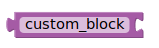
\includegraphics[width=0.2\textwidth]{img/CustomBlock.png}
\caption{Bloque personalizazdo} \label{fig:customblock}
\end{figure}

% BLENDER %
\section{Blender}
\label{sec:blender}
\textit{Blender} es un programa libre dedicado al diseño y animación 3D. 

\subsection{Modelos 3D}
% GESTORES DE PAQUETES %
\section{Gestores de paquetes}
\label{sec:gest}
\subsection{NPM}
\subsection{WebPack}

% WEBSIM %
\section{WebSim}

\textit{Websim} es un simulador robótico diseñado para enseñar conceptos básicos de tecnología e iniciar a niños en robótica y programación de robots. 
\subsection{Descripción}
El simulador hace uso del entorno \textit{A-Frame} y permite conectar un editor de texto o un editor de bloques para poder programar en \textit{JavaScript} o \textit{Blockly} y conectar este código con el robot simulado. 

\subsection{Drivers}
\begin{table}[h!]
  \begin{center}
    \caption{Métodos (HAL API) de los motores del robot.}
    \vspace{0.5cm}
    \label{tab:tabla-motores}
    \begin{tabular}{|c|c|} 
    \hline
      \textbf{Método} & \textbf{Descripción}\\
      \hline
.setV(integer) & \begin{tabular}[c]{@{}c@{}}Mueve hacia delante o atrás el robot.\\\end{tabular} \\ \hline
.setW(integer) & \begin{tabular}[c]{@{}c@{}}Hace girar al robot.\\\end{tabular} \\ \hline
.move(integer, integer) & \begin{tabular}[c]{@{}c@{}}Mueve el robot hacia delante/atrás y gira al mismo tiempo.\\ \end{tabular} \\ \hline
.getV() & \begin{tabular}[c]{@{}c@{}}Obtener la velocidad lineal configurada en el robot.\\ \end{tabular} \\ \hline
.getW() & \begin{tabular}[c]{@{}c@{}}Obtener la velocidad angular configurada en el robot.\\ \end{tabular} \\ \hline
    \end{tabular}
  \end{center}
\end{table}

